% Created 2015-01-26 Mon 17:16
\documentclass[11pt]{book}
\usepackage{graphicx}
\usepackage{xcolor}
\usepackage{xeCJK}
\setCJKmainfont{SimSun}
\usepackage{longtable}
\usepackage{float}
\usepackage{textcomp}
\usepackage{geometry}
\geometry{left=0cm,right=0cm,top=0cm,bottom=0cm}
\usepackage{multirow}
\usepackage{multicol}
\usepackage{listings}
\usepackage{algorithm}
\usepackage{algorithmic}
\usepackage{latexsym}
\usepackage{natbib}
\usepackage{fancyhdr}
\usepackage[xetex,colorlinks=true,CJKbookmarks=true,linkcolor=blue,urlcolor=blue,menucolor=blue]{hyperref}


\lstset{language=Java,numbers=left,numberstyle=\tiny,basicstyle=\ttfamily\small,tabsize=4,frame=none,escapeinside=``,extendedchars=false,keywordstyle=\color{blue!70},commentstyle=\color{red!55!green!55!blue!55!},rulesepcolor=\color{red!20!green!20!blue!20!}}
\author{deepwaterooo}
\date{\today}
\title{LeetCode Summary}
\hypersetup{
  pdfkeywords={},
  pdfsubject={},
  pdfcreator={Emacs 24.3.1 (Org mode 8.2.7c)}}
\begin{document}

\maketitle
\tableofcontents


\chapter{数组 Array}
\label{sec-1}
\section{Easy}
\label{sec-1-1}
\subsection{Remove Element}
\label{sec-1-1-1}
\subsection{Remove Duplicates from Sorted Array}
\label{sec-1-1-2}
\subsection{Plus One}
\label{sec-1-1-3}
\subsection{Pascal's Triangle}
\label{sec-1-1-4}
\subsection{Pascal's Triangle II}
\label{sec-1-1-5}
\subsection{Merge Sorted Array}
\label{sec-1-1-6}
\subsection{Majority Element}
\label{sec-1-1-7}
\section{Medium}
\label{sec-1-2}
\subsection{Two Sum}
\label{sec-1-2-1}
\subsection{3Sum Closest}
\label{sec-1-2-2}
\subsection{Container With Most Water}
\label{sec-1-2-3}
\subsection{Set Matrix Zeroes}
\label{sec-1-2-4}
\subsection{Minimum Path Sum}
\label{sec-1-2-5}
\subsection{Search Insert Position}
\label{sec-1-2-6}
\subsection{Unique Paths}
\label{sec-1-2-7}
\subsection{Search in Rotated Sorted Array II}
\label{sec-1-2-8}
\subsection{Search for a Range}
\label{sec-1-2-9}
\subsection{Search a 2D Matrix}
\label{sec-1-2-10}
\subsection{Rotate Image}
\label{sec-1-2-11}
\subsection{3Sum}
\label{sec-1-2-12}
\subsection{4Sum}
\label{sec-1-2-13}
\subsection{Remove Duplicates from Sorted Array II}
\label{sec-1-2-14}
\subsection{Best Time to Buy and Sell Stock II}
\label{sec-1-2-15}
\subsection{Unique Paths II}
\label{sec-1-2-16}
\subsection{Best Time to Buy and Sell Stock}
\label{sec-1-2-17}
\subsection{Next Permutation}
\label{sec-1-2-18}
\subsection{Missing Ranges}
\label{sec-1-2-19}
\subsection{Find Minimum in Rotated Sorted Array}
\label{sec-1-2-20}
\subsection{Combination Sum II}
\label{sec-1-2-21}
\subsection{Two Sum II - Input array is sorted}
\label{sec-1-2-22}
\subsection{Triangle}
\label{sec-1-2-23}
\subsection{Maximum Subarray}
\label{sec-1-2-24}
\subsection{Maximum Product Subarray}
\label{sec-1-2-25}
\subsection{Word Search}
\label{sec-1-2-26}
\subsection{Combination Sum}
\label{sec-1-2-27}
\subsection{Subsets}
\label{sec-1-2-28}
\subsection{Subsets II}
\label{sec-1-2-29}
\subsection{Jump Game}
\label{sec-1-2-30}
\subsection{Spiral Matrix}
\label{sec-1-2-31}
\subsection{Spiral Matrix II}
\label{sec-1-2-32}
\subsection{Sort Colors}
\label{sec-1-2-33}
\subsection{Find Peak Element}
\label{sec-1-2-34}
\section{Hard}
\label{sec-1-3}
\subsection{Trapping Rain Water}
\label{sec-1-3-1}
\subsection{Find Minimum in Rotated Sorted Array II}
\label{sec-1-3-2}
\subsection{Insert Interval}
\label{sec-1-3-3}
\subsection{Jump Game II}
\label{sec-1-3-4}
\subsection{Largest Rectangle in Histogram}
\label{sec-1-3-5}
\subsection{Longest Consecutive Sequence}
\label{sec-1-3-6}
\subsection{First Missing Positive}
\label{sec-1-3-7}
\subsection{Median of Two Sorted Arrays}
\label{sec-1-3-8}
\subsection{Merge Intervals}
\label{sec-1-3-9}
\subsection{Word Ladder II}
\label{sec-1-3-10}
\subsection{Best Time to Buy and Sell Stock III}
\label{sec-1-3-11}
\subsection{Search in Rotated Sorted Array}
\label{sec-1-3-12}
\subsection{Maximal Rectangle}
\label{sec-1-3-13}
\section{Others}
\label{sec-1-4}
\subsection{Construct Binary Tree from Inorder and Postorder Traversal}
\label{sec-1-4-1}
\subsection{Construct Binary Tree from Preorder and Inorder Traversal}
\label{sec-1-4-2}
\chapter{字符串 String}
\label{sec-2}
\section{Easy}
\label{sec-2-1}
\subsection{Valid Parentheses}
\label{sec-2-1-1}
\subsection{Add Binary}
\label{sec-2-1-2}
\subsection{Compare Version Numbers}
\label{sec-2-1-3}
\subsection{Count and Say}
\label{sec-2-1-4}
\subsection{Longest Common Prefix}
\label{sec-2-1-5}
\subsection{Roman to Integer}
\label{sec-2-1-6}
\subsection{Valid Palindrome}
\label{sec-2-1-7}
\subsection{Read N Characters Given Read4}
\label{sec-2-1-8}
\subsection{Implement strStr()}
\label{sec-2-1-9}
\subsection{ZigZag Conversion}
\label{sec-2-1-10}
\subsection{String to Integer (atoi)}
\label{sec-2-1-11}
\subsection{Length of Last Word}
\label{sec-2-1-12}
\section{Medium}
\label{sec-2-2}
\subsection{Restore IP Addresses}
\label{sec-2-2-1}
\subsection{Anagrams}
\label{sec-2-2-2}
\subsection{Integer to Roman}
\label{sec-2-2-3}
\subsection{Multiply Strings}
\label{sec-2-2-4}
\subsection{One Edit Distance}
\label{sec-2-2-5}
\subsection{Longest Palindromic Substring}
\label{sec-2-2-6}
\subsection{Letter Combinations of a Phone Number}
\label{sec-2-2-7}
\subsection{Decode Ways}
\label{sec-2-2-8}
\subsection{Longest Substring Without Repeating Characters}
\label{sec-2-2-9}
\subsection{Generate Parentheses}
\label{sec-2-2-10}
\subsection{Reverse Words in a String}
\label{sec-2-2-11}
\subsection{Simplify Path}
\label{sec-2-2-12}
\section{Hard}
\label{sec-2-3}
\subsection{Edit Distance}
\label{sec-2-3-1}
\subsection{Minimum Window Substring}
\label{sec-2-3-2}
\subsection{Longest Valid Parentheses}
\label{sec-2-3-3}
\subsection{Longest Substring with At Most Two Distinct Characters}
\label{sec-2-3-4}
\subsection{Read N Characters Given Read4 II - Call multiple times}
\label{sec-2-3-5}
\subsection{Regular Expression Matching}
\label{sec-2-3-6}
\subsection{Interleaving String}
\label{sec-2-3-7}
\subsection{Wildcard Matching}
\label{sec-2-3-8}
\subsection{Scramble String}
\label{sec-2-3-9}
\subsection{Distinct Subsequences}
\label{sec-2-3-10}
\subsection{Substring with Concatenation of All Words}
\label{sec-2-3-11}
\subsection{Text Justification}
\label{sec-2-3-12}
\subsection{Valid Number}
\label{sec-2-3-13}
\subsection{Word Ladder II}
\label{sec-2-3-14}

\chapter{Linked List}
\label{sec-3}
\section{Easy}
\label{sec-3-1}
\subsection{Remove Nth Node From End of List}
\label{sec-3-1-1}
\subsection{Remove Duplicates from Sorted List}
\label{sec-3-1-2}
\subsection{Merge Two Sorted Lists}
\label{sec-3-1-3}
\subsection{Intersection of Two Linked Lists}
\label{sec-3-1-4}
\section{Medium}
\label{sec-3-2}
\subsection{Reverse Linked List II}
\label{sec-3-2-1}
\subsection{Reorder List}
\label{sec-3-2-2}
\subsection{Convert Sorted List to Binary Search Tree}
\label{sec-3-2-3}
\subsection{Rotate List}
\label{sec-3-2-4}
\subsection{Remove Duplicates from Sorted List II}
\label{sec-3-2-5}
\subsection{Sort List}
\label{sec-3-2-6}
\subsection{Insertion Sort List}
\label{sec-3-2-7}
\subsection{Swap Nodes in Pairs}
\label{sec-3-2-8}
\subsection{Linked List Cycle}
\label{sec-3-2-9}
\subsection{Linked List Cycle II}
\label{sec-3-2-10}
\subsection{Add Two Numbers}
\label{sec-3-2-11}
\subsection{Partition List}
\label{sec-3-2-12}
\section{Hard}
\label{sec-3-3}
\subsection{Copy List with Random Pointer}
\label{sec-3-3-1}
\subsection{Merge k Sorted Lists}
\label{sec-3-3-2}
\subsection{Reverse Nodes in k-Group}
\label{sec-3-3-3}

\chapter{树 Binary Tree, Binary Search Tree}
\label{sec-4}
\section{二叉树的遍历}
\label{sec-4-1}
\subsection{Binary Tree Preorder Traversal}
\label{sec-4-1-1}
\subsection{Binary Tree Inorder Traversal}
\label{sec-4-1-2}
\subsection{Binary Tree Postorder Traversal}
\label{sec-4-1-3}
\subsection{Binary Tree Level Order Traversal}
\label{sec-4-1-4}
\subsection{Binary Tree Level Order Traversal II}
\label{sec-4-1-5}
\subsection{Binary Tree Zigzag Level Order Traversal}
\label{sec-4-1-6}
\subsection{Recover Binary Search Tree}
\label{sec-4-1-7}

\subsection{Same Tree}
\label{sec-4-1-8}
\subsection{Symmetric Tree}
\label{sec-4-1-9}
\subsection{Balanced Binary Tree}
\label{sec-4-1-10}
\subsection{Flatten Binary Tree to Linked List}
\label{sec-4-1-11}
\subsection{Populating Next Right Pointers in Each Node II}
\label{sec-4-1-12}
\section{二叉树的构建}
\label{sec-4-2}
\subsection{Construct Binary Tree from Preorder and Inorder Traversal}
\label{sec-4-2-1}
\subsection{Construct Binary Tree from Inorder and Postorder Traversal}
\label{sec-4-2-2}
\section{二叉树查找}
\label{sec-4-3}
\subsection{Unique Binary Search Trees}
\label{sec-4-3-1}
\subsection{Unique Binary Search Trees II}
\label{sec-4-3-2}
\subsection{Validate Binary Search Tree}
\label{sec-4-3-3}
\subsection{Convert Sorted Array to Binary Search Tree}
\label{sec-4-3-4}
\subsection{Convert Sorted List to Binary Search Tree}
\label{sec-4-3-5}
\section{二叉树递归}
\label{sec-4-4}
\subsection{Minimum Depth of Binary Tree}
\label{sec-4-4-1}
\subsection{Maximum Depth of Binary Tree}
\label{sec-4-4-2}
\subsection{Path Sum}
\label{sec-4-4-3}
\subsection{Path Sum II}
\label{sec-4-4-4}
\subsection{Binary Tree Maximum Path Sum}
\label{sec-4-4-5}
\subsection{Populating Next Right Pointers in Each Node}
\label{sec-4-4-6}

\subsection{Sum Root to Leaf Numbers}
\label{sec-4-4-7}
\subsection{Binary Tree Upside Down: this 2 ?}
\label{sec-4-4-8}
\subsection{Binary Search Tree Iterator}
\label{sec-4-4-9}
\chapter{栈和队列}
\label{sec-5}
\section{栈}
\label{sec-5-1}
\section{Easy}
\label{sec-5-2}
\subsection{Valid Parentheses}
\label{sec-5-2-1}
\subsection{Min Stack}
\label{sec-5-2-2}
\section{Medium}
\label{sec-5-3}
\subsection{Binary Tree Inorder Traversal}
\label{sec-5-3-1}
\subsection{Binary Search Tree Iterator}
\label{sec-5-3-2}
\subsection{Evaluate Reverse Polish Notation}
\label{sec-5-3-3}
\subsection{Simplify Path}
\label{sec-5-3-4}
\subsection{Binary Tree Preorder Traversal}
\label{sec-5-3-5}
\subsection{Binary Tree Zigzag Level Order Traversal}
\label{sec-5-3-6}
\section{Hard}
\label{sec-5-4}
\subsection{Binary Tree Postorder Traversal}
\label{sec-5-4-1}
\subsection{Largest Rectangle in Histogram}
\label{sec-5-4-2}
\subsection{Trapping Rain Water}
\label{sec-5-4-3}
\subsection{Maximal Rectangle}
\label{sec-5-4-4}
\section{队列}
\label{sec-5-5}
\subsection{}
\label{sec-5-5-1}
\section{Heap:}
\label{sec-5-6}
\subsection{Merge k sorted List}
\label{sec-5-6-1}
Merge k sorted linked lists and return it as one sorted list. Analyze and describe its complexity.

\textbf{Tags}: Divide and Conquer, Linked List, Heap
\lstset{language=java,label= ,caption= ,numbers=none}
\begin{lstlisting}
public ListNode mergeTwoLists(ListNode l1, ListNode l2) {
    if (l1 == null) return l2;
    if (l2 == null) return l1;
    ListNode result;
    if (l1.val < l2.val) {
        result = l1;
        l1 = l1.next;
        result.next = null;
    } else {
        result = l2;
        l2 = l2.next;
        result.next = null;
    }
    ListNode curr = result;
    while (l1 != null && l2 != null) {
        if (l1.val < l2.val) {
            curr.next = l1;
            curr = curr.next;
            l1 = l1.next;
            curr.next = null;
        } else {
            curr.next = l2;
            curr = curr.next;
            l2 = l2.next;
            curr.next = null;
        }
    }
    if (l1 == null && l2 == null)
        return result;
    l1 = (l1 == null) ? l2 : l1;
    curr.next = l1;
    return result;
}

public ListNode mergeKLists(List<ListNode> lists) {
    if (lists.size() == 0) return null;
    if (lists.size() == 1) return lists.get(0);
    if (lists.size() == 2) return mergeTwoLists(lists.get(0), lists.get(1));
    return mergeTwoLists((mergeKLists(lists.subList(0, lists.size() / 2))),
                         (mergeKLists(lists.subList(lists.size() / 2, lists.size()))));
}
\end{lstlisting}

\chapter{Hash Table}
\label{sec-6}
\section{Easy}
\label{sec-6-1}
\subsection{Valid Sudoku}
\label{sec-6-1-1}
\subsection{Two Sum III}
\label{sec-6-1-2}
\section{Medium}
\label{sec-6-2}
\subsection{Two Sum}
\label{sec-6-2-1}
\subsection{4Sum}
\label{sec-6-2-2}
\subsection{Binary Tree Inorder Traversal}
\label{sec-6-2-3}
\subsection{Fraction to Recurring Decimal}
\label{sec-6-2-4}
\subsection{Single Number}
\label{sec-6-2-5}
\subsection{Anagrams}
\label{sec-6-2-6}
\subsection{Longest Substring Without Repeating Characters}
\label{sec-6-2-7}
\section{Hard}
\label{sec-6-3}
\subsection{Minimum Window Substring}
\label{sec-6-3-1}
\subsection{Maximal Rectangle}
\label{sec-6-3-2}
\subsection{Copy List with Random Pointer}
\label{sec-6-3-3}
\subsection{Sudoku Solver}
\label{sec-6-3-4}
\subsection{Max Points on a Line}
\label{sec-6-3-5}
\subsection{Substring with Concatenation of All Words}
\label{sec-6-3-6}
\subsection{Longest Substring with At Most Two Distinct Characters}
\label{sec-6-3-7}
\chapter{广度优先搜索 Breadth First Search}
\label{sec-7}
\section{Easy}
\label{sec-7-1}
\subsection{Binary Tree Level Order Traversal}
\label{sec-7-1-1}
\subsection{Binary Tree Level Order Traversal II}
\label{sec-7-1-2}
\section{Medium}
\label{sec-7-2}
\subsection{Word Ladder}
\label{sec-7-2-1}
Given two words (start and end), and a dictionary, find the length of shortest transformation sequence from start to end, such that:
\begin{itemize}
\item Only one letter can be changed at a time
\item Each intermediate word must exist in the dictionary
\end{itemize}
For example,

Given:
\lstset{language=java,label= ,caption= ,numbers=none}
\begin{lstlisting}
start = "hit"
end = "cog"
dict = ["hot","dot","dog","lot","log"]
As one shortest transformation is "hit" -> "hot" -> "dot" -> "dog" -> "cog",
return its length 5.
\end{lstlisting}
Note:
\begin{itemize}
\item Return 0 if there is no such transformation sequence.
\item All words have the same length.
\item All words contain only lowercase alphabetic characters.
\end{itemize}
\subsection{Surrounded Regions}
\label{sec-7-2-2}
\subsection{Clone Graph}
\label{sec-7-2-3}
\subsection{Binary Tree Zigzag Level Order Traversal}
\label{sec-7-2-4}
\subsection{Minimum Depth of Binary Tree}
\label{sec-7-2-5}

\section{Hard}
\label{sec-7-3}
\subsection{Word Ladder II}
\label{sec-7-3-1}

\chapter{深度优先搜索 Depth First Search}
\label{sec-8}
\section{Easy}
\label{sec-8-1}
\subsection{Path Sum}
\label{sec-8-1-1}
\subsection{Balanced Binary Tree}
\label{sec-8-1-2}
\subsection{Same Tree}
\label{sec-8-1-3}
\subsection{Symmetric Tree}
\label{sec-8-1-4}
\subsection{Maximum Depth of Binary Tree}
\label{sec-8-1-5}
\section{Medium}
\label{sec-8-2}
\subsection{Sum Root to Leaf Numbers}
\label{sec-8-2-1}
\subsection{Convert Sorted List to Binary Search Tree}
\label{sec-8-2-2}
\subsection{Convert Sorted Array to Binary Search Tree}
\label{sec-8-2-3}
\subsection{Construct Binary Tree from Preorder and Inorder Traversal}
\label{sec-8-2-4}
\subsection{Construct Binary Tree from Inorder and Postorder Traversal}
\label{sec-8-2-5}
\subsection{Clone Graph}
\label{sec-8-2-6}
\subsection{Flatten Binary Tree to Linked List}
\label{sec-8-2-7}
\subsection{Populating Next Right Pointers in Each Node}
\label{sec-8-2-8}
\subsection{Validate Binary Search Tree}
\label{sec-8-2-9}
\subsection{Path Sum II}
\label{sec-8-2-10}
\section{Hard}
\label{sec-8-3}
\subsection{Recover Binary Search Tree}
\label{sec-8-3-1}
\subsection{Populating Next Right Pointers in Each Node II}
\label{sec-8-3-2}
\subsection{Binary Tree Maximum Path Sum}
\label{sec-8-3-3}
\chapter{排序}
\label{sec-9}
\section{Medium}
\label{sec-9-1}
\subsection{Sort Colors}
\label{sec-9-1-1}
\subsection{Sort List}
\label{sec-9-1-2}
\subsection{Largest Number}
\label{sec-9-1-3}
\section{Hard}
\label{sec-9-2}
\subsection{Insertion Sort List}
\label{sec-9-2-1}
\subsection{Maximum Gap}
\label{sec-9-2-2}
\subsection{Merge Intervals}
\label{sec-9-2-3}
\subsection{Insert Interval}
\label{sec-9-2-4}

\chapter{查找 Binary Search}
\label{sec-10}
\section{Medium}
\label{sec-10-1}
\subsection{Sqrt(x)}
\label{sec-10-1-1}
\subsection{Divide Two Integers}
\label{sec-10-1-2}
\subsection{Search in Rotated Sorted Array II}
\label{sec-10-1-3}
\subsection{Two Sum II - Input array is sorted}
\label{sec-10-1-4}
\subsection{Pow(x, n)}
\label{sec-10-1-5}
\subsection{Search for a Range}
\label{sec-10-1-6}
\subsection{Search a 2D Matrix}
\label{sec-10-1-7}
\subsection{Find Minimum in Rotated Sorted Array}
\label{sec-10-1-8}
\subsection{Search Insert Position}
\label{sec-10-1-9}
\subsection{Find Peak Element}
\label{sec-10-1-10}
\section{Hard}
\label{sec-10-2}
\subsection{Median of Two Sorted Arrays}
\label{sec-10-2-1}
\subsection{Dungeon Game}
\label{sec-10-2-2}
\subsection{Find Minimum in Rotated Sorted Array II}
\label{sec-10-2-3}
\subsection{Search in Rotated Sorted Array}
\label{sec-10-2-4}
\chapter{暴力枚举法}
\label{sec-11}
\section{}
\label{sec-11-1}
\subsection{}
\label{sec-11-1-1}
\chapter{分治法 Divide and Conqure}
\label{sec-12}
\section{Easy}
\label{sec-12-1}
\subsection{Majority Element}
\label{sec-12-1-1}
\section{Medium}
\label{sec-12-2}
\subsection{Maximum Subarray}
\label{sec-12-2-1}
\section{Hard}
\label{sec-12-3}
\subsection{Merge K sorted List}
\label{sec-12-3-1}
\subsection{Median of Two Sorted Array}
\label{sec-12-3-2}
\chapter{贫心法 Greedy Search}
\label{sec-13}
\section{Medium}
\label{sec-13-1}
\subsection{Gas Station}
\label{sec-13-1-1}
\subsection{Best Time to Buy and Sell Stock II}
\label{sec-13-1-2}
\subsection{Jump Game}
\label{sec-13-1-3}
\section{Hard}
\label{sec-13-2}
\subsection{Jump Game II}
\label{sec-13-2-1}
\subsection{Candy}
\label{sec-13-2-2}
\subsection{Wildcard Matching}
\label{sec-13-2-3}
\subsection{}
\label{sec-13-2-4}

\chapter{动态归划 Dynamic Programming}
\label{sec-14}
\section{Easy}
\label{sec-14-1}
\subsection{Climbing Stairs}
\label{sec-14-1-1}
You are climbing a stair case. It takes n steps to reach to the top.

Each time you can either climb 1 or 2 steps. In how many distinct ways
can you climb to the top?
\begin{enumerate}
\item O(n)
\label{sec-14-1-1-1}
\lstset{language=java,label= ,caption= ,numbers=none}
\begin{lstlisting}
public int climbStairs(int n) {
    int [] res = new int[n + 1];
    res[0] = 1; // 1 stair
    res[1] = 2; // 2 stair
    for (int i = 2; i < n; i++) 
        res[i] = res[i - 2] + res[i - 1];
    return res[n - 1];
}
\end{lstlisting}
Considering odd and even, 实现滚动数组
\lstset{language=java,label= ,caption= ,numbers=none}
\begin{lstlisting}
public int climbStairs(int n){
    if(n <= 0) return 0;
    int [] stairs = {1, 2};
    for(int i = 2;i < n; i++)
        stairs[i % 2] = stairs[0] + stairs[1];
    return n % 2 == 0 ? stairs[1] : stairs[0];
}
\end{lstlisting}
\item O( log(n) )
\label{sec-14-1-1-2}

\url{https://oj.leetcode.com/discuss/11211/o-log-n-solution-with-matrix-multiplication}

I saw most solutions posted in discussion are DP with runtime O(n) and O(1) space which is accepted by OJ.

The only O(log(n)) solution so far is lucastan's using Binet's formula.

There actually is a matrix multiplication solution which also runs in O(log(n)). It basically calculates fibonacci numbers by power of matrix ((0, 1), (1, 1)) \^{} (n-1).

\lstset{language=java,label= ,caption= ,numbers=none}
\begin{lstlisting}
private int[][] pow(int[][] a, int n) {
    int[][] ret = {{1, 0}, {0, 1}};
    while (n > 0) {
        if ((n & 1) == 1) 
            ret = multiply(ret, a);
        n >>= 1;
        a = multiply(a, a);
    }
    return ret;
}

private int[][] multiply(int[][] a, int[][] b) {
    int[][] c = new int[2][2];
    for (int i = 0; i < 2; i++) 
        for (int j = 0; j < 2; j++) 
            c[i][j] = a[i][0] * b[0][j] + a[i][1] * b[1][j];
    return c;
}

public int climbStairs(int n) {
    int[][] a = {{0, 1}, {1, 1}};
    int[][] m = pow(a, n - 1);
    return m[0][1] + m[1][1];
}
\end{lstlisting}
\end{enumerate}
\section{Medium}
\label{sec-14-2}
\subsection{Unique Path}
\label{sec-14-2-1}
\subsection{Unique Path II}
\label{sec-14-2-2}
\subsection{Unique Binary Search Tree}
\label{sec-14-2-3}
\subsection{Unique Binary Search Tree II}
\label{sec-14-2-4}
\subsection{Minimum Path Sum}
\label{sec-14-2-5}
\subsection{Maximum Sum Subarray}
\label{sec-14-2-6}
\subsection{Maximum Product Subarray}
\label{sec-14-2-7}
\subsection{Decode Ways}
\label{sec-14-2-8}
\subsection{Triangle}
\label{sec-14-2-9}
\subsection{Word Break}
\label{sec-14-2-10}
Given a string s and a dictionary of words dict, determine if s can be segmented into a space-separated sequence of one or more dictionary words.

For example, given
\lstset{language=java,label= ,caption= ,numbers=none}
\begin{lstlisting}
s = "leetcode",
dict = ["leet", "code"].
Return true because "leetcode" can be segmented as "leet code".
\end{lstlisting}
\subsection{Best Time to Buy and Sell Stock}
\label{sec-14-2-11}
\section{Hard}
\label{sec-14-3}
\subsection{Best Time to Buy and Sell Stock III}
\label{sec-14-3-1}
\subsection{Longest Valid Parentheses}
\label{sec-14-3-2}

\subsection{Coins in a Line}
\label{sec-14-3-3}
\subsection{Word Break II}
\label{sec-14-3-4}
\subsection{Maximum Rectangle}
\label{sec-14-3-5}
\subsection{Edit Distance}
\label{sec-14-3-6}
\subsection{Distinct Subsequence}
\label{sec-14-3-7}
\subsection{Palindrome Partitioning II}
\label{sec-14-3-8}
Given a string s, partition s such that every substring of the partition is a palindrome.

Return the minimum cuts needed for a palindrome partitioning of s.

For example, 
\lstset{language=java,label= ,caption= ,numbers=none}
\begin{lstlisting}
given s = "aab",
Return 1 since the palindrome partitioning ["aa","b"] could be produced using 1 cut.
\end{lstlisting}

\subsection{Interleaving String}
\label{sec-14-3-9}
\subsection{Scramble String}
\label{sec-14-3-10}
\subsection{Regular Expression Matching}
\label{sec-14-3-11}
\subsection{Wildcard Matching}
\label{sec-14-3-12}
\chapter{Two Pointers and Sliding Window}
\label{sec-15}
\section{Easy}
\label{sec-15-1}
\subsection{Valid Palindrome}
\label{sec-15-1-1}
\subsection{Remove Nth Node From End of List}
\label{sec-15-1-2}
\subsection{Remove Element}
\label{sec-15-1-3}
\subsection{Remove Duplicates from Sorted Array}
\label{sec-15-1-4}
\subsection{Merge Sorted Array}
\label{sec-15-1-5}
\subsection{Implement strStr()}
\label{sec-15-1-6}
\section{Medium}
\label{sec-15-2}
\subsection{3Sum}
\label{sec-15-2-1}
\subsection{4Sum}
\label{sec-15-2-2}
\subsection{Container With Most Water}
\label{sec-15-2-3}
\subsection{Remove Duplicates from Sorted Array II}
\label{sec-15-2-4}
\subsection{Partition List}
\label{sec-15-2-5}
\subsection{Two Sum II - Input array is sorted}
\label{sec-15-2-6}
\subsection{Linked List Cycle II}
\label{sec-15-2-7}
\subsection{Longest Substring Without Repeating Characters}
\label{sec-15-2-8}
\subsection{3Sum Closest}
\label{sec-15-2-9}
\subsection{Linked List Cycle}
\label{sec-15-2-10}
\subsection{Sort Colors}
\label{sec-15-2-11}
\subsection{Rotate List}
\label{sec-15-2-12}
\section{Hard}
\label{sec-15-3}
\subsection{Trapping Rain Water}
\label{sec-15-3-1}
\subsection{Longest Substring with At Most Two Distinct Characters}
\label{sec-15-3-2}
\subsection{Substring with Concatenation of All Words}
\label{sec-15-3-3}
\subsection{Minimum Window Substring}
\label{sec-15-3-4}
\chapter{Backtracing and Recursion}
\label{sec-16}
\section{排列}
\label{sec-16-1}
\subsection{Permutation}
\label{sec-16-1-1}
Given a collection of numbers, return all possible permutations.

For example,
\lstset{language=java,label= ,caption= ,numbers=none}
\begin{lstlisting}
[1,2,3] have the following permutations:
[1,2,3], [1,3,2], [2,1,3], [2,3,1], [3,1,2], and [3,2,1].
\end{lstlisting}
\subsection{Permutation II}
\label{sec-16-1-2}
Given a collection of numbers that might contain duplicates, return all possible unique permutations.

For example,
\lstset{language=java,label= ,caption= ,numbers=none}
\begin{lstlisting}
[1,1,2] have the following unique permutations:
[1,1,2], [1,2,1], and [2,1,1].
\end{lstlisting}
\subsection{Permutation Sequence}
\label{sec-16-1-3}
The set [1,2,3,…,n] contains a total of n! unique permutations.

By listing and labeling all of the permutations in order, We get the following sequence (ie, for n = 3):
\lstset{language=java,label= ,caption= ,numbers=none}
\begin{lstlisting}
"123"
"132"
"213"
"231"
"312"
"321"
\end{lstlisting}
Given n and k, return the kth permutation sequence.

Note: Given n will be between 1 and 9 inclusive.
\section{组合}
\label{sec-16-2}
\subsection{Combinationas}
\label{sec-16-2-1}
Given two integers n and k, return all possible combinations of k numbers out of 1 \ldots{} n.

For example,

If n = 4 and k = 2, a solution is:
\lstset{language=java,label= ,caption= ,numbers=none}
\begin{lstlisting}
[
  [2,4],
  [3,4],
  [2,3],
  [1,2],
  [1,3],
  [1,4],
]
\end{lstlisting}
\subsection{Combination Sum}
\label{sec-16-2-2}
Given a set of candidate numbers (C) and a target number (T), find all unique combinations in C where the candidate numbers sums to T.

The same repeated number may be chosen from C unlimited number of times.

Note:
\begin{itemize}
\item All numbers (including target) will be positive integers.
\item Elements in a combination (a1, a2, … , ak) must be in non-descending order. (ie, a1 ≤ a2 ≤ … ≤ ak).
\item The solution set must not contain duplicate combinations.
\end{itemize}

For example, given candidate set 2,3,6,7 and target 7, 

A solution set is: 
\lstset{language=java,label= ,caption= ,numbers=none}
\begin{lstlisting}
[7] 
[2, 2, 3]
\end{lstlisting}
\subsection{Combination Sum II}
\label{sec-16-2-3}
Given a collection of candidate numbers (C) and a target number (T), find all unique combinations in C where the candidate numbers sums to T.

Each number in C may only be used once in the combination.

Note:
\begin{itemize}
\item All numbers (including target) will be positive integers.
\item Elements in a combination (a1, a2, … , ak) must be in non-descending order. (ie, a1 ≤ a2 ≤ … ≤ ak).
\item The solution set must not contain duplicate combinations.
\end{itemize}
For example, given candidate set 10,1,2,7,6,1,5 and target 8, 

A solution set is: 
\lstset{language=java,label= ,caption= ,numbers=none}
\begin{lstlisting}
[1, 7] 
[1, 2, 5] 
[2, 6] 
[1, 1, 6]
\end{lstlisting}
\section{Subsets}
\label{sec-16-3}
\subsection{Subsets: Bit Manipulation}
\label{sec-16-3-1}
Given a set of distinct integers, S, return all possible subsets.

Note:
\begin{itemize}
\item Elements in a subset must be in non-descending order.
\item The solution set must not contain duplicate subsets.
\end{itemize}
For example,

If S = [1,2,3], a solution is:
\lstset{language=java,label= ,caption= ,numbers=none}
\begin{lstlisting}
[
  [3],
  [1],
  [2],
  [1,2,3],
  [1,3],
  [2,3],
  [1,2],
  []
]
\end{lstlisting}
\textbf{Tags:} Array Backtracking, Bit Manipulation
\subsection{Subsets II}
\label{sec-16-3-2}
Given a collection of integers that might contain duplicates, S, return all possible subsets.

Note:
\begin{itemize}
\item Elements in a subset must be in non-descending order.
\item The solution set must not contain duplicate subsets.
\end{itemize}
For example,

If S = [1,2,2], a solution is:
\lstset{language=java,label= ,caption= ,numbers=none}
\begin{lstlisting}
[
  [2],
  [1],
  [1,2,2],
  [2,2],
  [1,2],
  []
]
\end{lstlisting}
\section{others with Recursion}
\label{sec-16-4}
\subsection{Letter Combinationas of Phone Number}
\label{sec-16-4-1}
Given a digit string, return all possible letter combinations that the number could represent.

A mapping of digit to letters (just like on the telephone buttons) is given below.

\begin{figure}[htb]
\centering
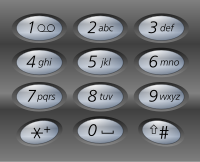
\includegraphics[width=.9\linewidth]{./pic/phoneNumber.png}
\caption{Letter Combinationas of Phone Number}
\end{figure}
\lstset{language=java,label= ,caption= ,numbers=none}
\begin{lstlisting}
Input:Digit string "23"
Output: ["ad", "ae", "af", "bd", "be", "bf", "cd", "ce", "cf"].
\end{lstlisting}
Note:

Although the above answer is in lexicographical order, your answer could be in any order you want.
\subsection{Restore IP Addresses}
\label{sec-16-4-2}
Given a string containing only digits, restore it by returning all possible valid IP address combinations.

For example:
\lstset{language=java,label= ,caption= ,numbers=none}
\begin{lstlisting}
Given "25525511135",
return ["255.255.11.135", "255.255.111.35"]. (Order does not matter)
\end{lstlisting}
\subsection{Generate Parentheses}
\label{sec-16-4-3}
Given n pairs of parentheses, write a function to generate all combinations of well-formed parentheses.

For example, given n = 3, a solution set is:
\lstset{language=java,label= ,caption= ,numbers=none}
\begin{lstlisting}
"((()))", "(()())", "(())()", "()(())", "()()()"
\end{lstlisting}
\subsection{Gray Code}
\label{sec-16-4-4}
The gray code is a binary numeral system where two successive values differ in only one bit.

Given a non-negative integer n representing the total number of bits in the code, print the sequence of gray code. A gray code sequence must begin with 0.

For example, given n = 2, return [0,1,3,2]. Its gray code sequence is:
\lstset{language=java,label= ,caption= ,numbers=none}
\begin{lstlisting}
00 - 0
01 - 1
11 - 3
10 - 2
\end{lstlisting}
Note:
\begin{itemize}
\item For a given n, a gray code sequence is not uniquely defined.
\item For example, [0,2,3,1] is also a valid gray code sequence according to the above definition.
\item For now, the judge is able to judge based on one instance of gray code sequence. Sorry about that.
\end{itemize}
\subsection{Word Search}
\label{sec-16-4-5}
Given a 2D board and a word, find if the word exists in the grid.

The word can be constructed from letters of sequentially adjacent cell, where "adjacent" cells are those horizontally or vertically neighboring. The same letter cell may not be used more than once.

For example,
\lstset{language=java,label= ,caption= ,numbers=none}
\begin{lstlisting}
Given board =
[
  ["ABCE"],
  ["SFCS"],
  ["ADEE"]
]
word = "ABCCED", -> returns true,
word = "SEE", -> returns true,
word = "ABCB", -> returns false.
\end{lstlisting}
\subsection{Palindrome Partitioning}
\label{sec-16-4-6}
Given a string s, partition s such that every substring of the partition is a palindrome.

Return all possible palindrome partitioning of s.

For example, 
\lstset{language=java,label= ,caption= ,numbers=none}
\begin{lstlisting}
given s = "aab",
Return
  [
    ["aa","b"],
    ["a","a","b"]
  ]
\end{lstlisting}
\subsection{N-Queens}
\label{sec-16-4-7}
The n-queens puzzle is the problem of placing n queens on an n×n chessboard such that no two queens attack each other.
\begin{figure}[htb]
\centering
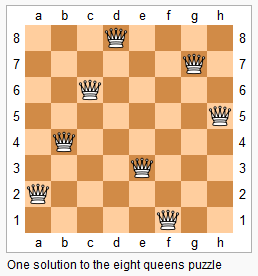
\includegraphics[width=.9\linewidth]{./pic/8-queens.png}
\caption{N-Queens}
\end{figure}

Given an integer n, return all distinct solutions to the n-queens puzzle.

Each solution contains a distinct board configuration of the n-queens' placement, where 'Q' and '.' both indicate a queen and an empty space respectively.

For example,

There exist two distinct solutions to the 4-queens puzzle:
\lstset{language=java,label= ,caption= ,numbers=none}
\begin{lstlisting}
[
 [".Q..",  // Solution 1
  "...Q",
  "Q...",
  "..Q."],

 ["..Q.",  // Solution 2
  "Q...",
  "...Q",
  ".Q.."]
]
\end{lstlisting}
\subsection{N-Queens II}
\label{sec-16-4-8}
Follow up for N-Queens problem.

Now, instead outputting board configurations, return the total number of distinct solutions.
\subsection{Sudoku Solver}
\label{sec-16-4-9}
Write a program to solve a Sudoku puzzle by filling the empty cells.

Empty cells are indicated by the character '.'.

You may assume that there will be only one unique solution.

\begin{figure}[htb]
\centering
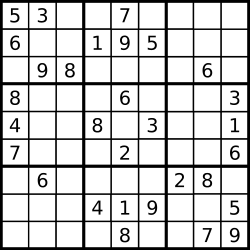
\includegraphics[width=.9\linewidth]{./pic/solveSudoku1.png}
\caption{Sudoku Solver 1}
\end{figure}
A sudoku puzzle\ldots{}

\begin{figure}[htb]
\centering
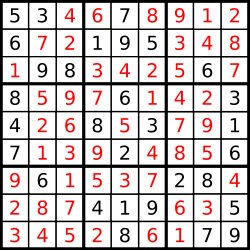
\includegraphics[width=.9\linewidth]{./pic/solveSudoku2.png}
\caption{Sudoku Solver 2}
\end{figure}
\ldots{}and its solution numbers marked in red.

\textbf{Tags:} Backtracking, Hash Table

\subsection{Regular Expression Matching}
\label{sec-16-4-10}
Implement regular expression matching with support for '.' and '*'.
\begin{itemize}
\item '.' Matches any single character.
\item '*' Matches zero or more of the preceding element.
\end{itemize}

The matching should cover the entire input string (not partial).

The function prototype should be:

bool isMatch(const char *s, const char *p)

Some examples:
\lstset{language=java,label= ,caption= ,numbers=none}
\begin{lstlisting}
isMatch("aa","a") → false
isMatch("aa","aa") → true
isMatch("aaa","aa") → false
isMatch("aa", "a*") → true
isMatch("aa", ".*") → true
isMatch("ab", ".*") → true
isMatch("aab", "c*a*b") → true
\end{lstlisting}
\textbf{Tags:} Dynamic Programming, Backtracking, String
\subsection{Wild Card Matching}
\label{sec-16-4-11}
Implement wildcard pattern matching with support for '?' and '*'.
\begin{itemize}
\item '?' Matches any single character.
\item '*' Matches any sequence of characters (including the empty sequence).
\end{itemize}

The matching should cover the entire input string (not partial).

The function prototype should be:

bool isMatch(const char *s, const char *p)

Some examples:
\lstset{language=java,label= ,caption= ,numbers=none}
\begin{lstlisting}
isMatch("aa","a") → false
isMatch("aa","aa") → true
isMatch("aaa","aa") → false
isMatch("aa", "*") → true
isMatch("aa", "a*") → true
isMatch("ab", "?*") → true
isMatch("aab", "c*a*b") → false
\end{lstlisting}
\textbf{Tags:} Dynamic Programming, Backtracking, Greedy, String
\subsection{Word Break II}
\label{sec-16-4-12}
Given a string s and a dictionary of words dict, add spaces in s to construct a sentence where each word is a valid dictionary word.

Return all such possible sentences.

For example, given
\lstset{language=java,label= ,caption= ,numbers=none}
\begin{lstlisting}
s = "catsanddog",
dict = ["cat", "cats", "and", "sand", "dog"].

A solution is ["cats and dog", "cat sand dog"].
\end{lstlisting}
\textbf{Tags:} Dynamic Programming Backtracking
\subsection{Word Ladder II}
\label{sec-16-4-13}
Given two words (start and end), and a dictionary, find all shortest transformation sequence(s) from start to end, such that:
\begin{itemize}
\item Only one letter can be changed at a time
\item Each intermediate word must exist in the dictionary
\end{itemize}
For example,
\lstset{language=java,label= ,caption= ,numbers=none}
\begin{lstlisting}
Given:
start = "hit"
end = "cog"
dict = ["hot","dot","dog","lot","log"]
Return
  [
    ["hit","hot","dot","dog","cog"],
    ["hit","hot","lot","log","cog"]
  ]
\end{lstlisting}
Note:
\begin{itemize}
\item All words have the same length.
\item All words contain only lowercase alphabetic characters.
\end{itemize}
\textbf{Tags:} Array, Backtracking, Breadth-first Search, String

\chapter{Bit Manipulation}
\label{sec-17}
\section{Easy}
\label{sec-17-1}
\subsection{Majority Element}
\label{sec-17-1-1}
\section{Medium}
\label{sec-17-2}
\subsection{Subsets: Bit Manipulation}
\label{sec-17-2-1}
Given a set of distinct integers, S, return all possible subsets.

Note:
\begin{itemize}
\item Elements in a subset must be in non-descending order.
\item The solution set must not contain duplicate subsets.
\end{itemize}
For example,
If S = [1,2,3], a solution is:
\lstset{language=java,label= ,caption= ,numbers=none}
\begin{lstlisting}
[
  [3],
  [1],
  [2],
  [1,2,3],
  [1,3],
  [2,3],
  [1,2],
  []
]
\end{lstlisting}
\textbf{Tags:} Array Backtracking, Bit Manipulation
\subsection{Single Number}
\label{sec-17-2-2}
\subsection{Single Number II}
\label{sec-17-2-3}
\chapter{图 Graphics}
\label{sec-18}
\section{Medium}
\label{sec-18-1}
\subsection{Clone Graph}
\label{sec-18-1-1}
Clone an undirected graph. Each node in the graph contains a label and a list of its neighbors.

OJ's undirected graph serialization:

Nodes are labeled uniquely.

We use \# as a separator for each node, and , as a separator for node label and each neighbor of the node.

As an example, consider the serialized graph \{0,1,2\#1,2\#2,2\}.

The graph has a total of three nodes, and therefore contains three parts as separated by \#.

\begin{enumerate}
\item First node is labeled as 0. Connect node 0 to both nodes 1 and 2.
\item Second node is labeled as 1. Connect node 1 to node 2.
\item Third node is labeled as 2. Connect node 2 to node 2 (itself), thus forming a self-cycle.
\end{enumerate}

Visually, the graph looks like the following:
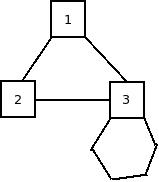
\includegraphics[width=.9\linewidth]{./pic/clonegraph.jpg}

\begin{enumerate}
\item 分析: 广度优先遍历或深度优先遍历都可以
\label{sec-18-1-1-1}
\item DFS: 时间复杂度O(n), 空间复杂度O(n)
\label{sec-18-1-1-2}
\lstset{language=java,label= ,caption= ,numbers=none}
\begin{lstlisting}
/**
 * Definition for undirected graph.
 * class UndirectedGraphNode {
 *     int label;
 *     List<UndirectedGraphNode> neighbors;
 *     UndirectedGraphNode(int x) { label = x; neighbors = new ArrayList<UndirectedGraphNode>(); }
 * };
 */
public UndirectedGraphNode cloneGraph(UndirectedGraphNode node) {
    if (node == null) return null;
    UndirectedGraphNode res = new UndirectedGraphNode(node.label);  // result head
    if (node.neighbors == null || node.neighbors.size() == 0) return res;

    Map<UndirectedGraphNode, UndirectedGraphNode> map = new HashMap<UndirectedGraphNode, UndirectedGraphNode>();
    Queue<UndirectedGraphNode> q = new LinkedList<UndirectedGraphNode>();
    q.add(node);                      // added first node, need add its all Neighbors as well
    map.put(node, res);

    List<UndirectedGraphNode> curNbr = new ArrayList<UndirectedGraphNode>();
    UndirectedGraphNode curr = null;
    while (!q.isEmpty()) {
        curr = q.poll();
        curNbr = curr.neighbors;                   // ori
        for (UndirectedGraphNode aNbr : curNbr) {  // for build connection among copies
            if (!map.containsKey(aNbr)) {
                UndirectedGraphNode acpNbr = new UndirectedGraphNode(aNbr.label);
                map.put(aNbr, acpNbr);
                map.get(curr).neighbors.add(acpNbr);
                q.add(aNbr);
            } else
                map.get(curr).neighbors.add(map.get(aNbr));                        
        }
    }
    return res;
}
\end{lstlisting}
\item BFS:
\label{sec-18-1-1-3}
\end{enumerate}
\section{Word Ladder, Word Ladder II: Backtracing}
\label{sec-18-2}
\subsection{Word Ladder}
\label{sec-18-2-1}
Given two words (start and end), and a dictionary, find the length of shortest transformation sequence from start to end, such that:
\begin{enumerate}
\item Only one letter can be changed at a time
\item Each intermediate word must exist in the dictionary
\end{enumerate}

For example,

Given:
start = "hit", end = "cog"

dict = ["hot","dot","dog","lot","log"]

As one shortest transformation is "hit" -> "hot" -> "dot" -> "dog" -> "cog",

return its length 5.

Note:
\begin{itemize}
\item Return 0 if there is no such transformation sequence.
\item All words have the same length.
\item All words contain only lowercase alphabetic characters.
\end{itemize}

\subsection{Word Ladder II}
\label{sec-18-2-2}
Given two words (start and end), and a dictionary, find all shortest transformation sequence(s) from start to end, such that:
\begin{enumerate}
\item Only one letter can be changed at a time
\item Each intermediate word must exist in the dictionary
\end{enumerate}
For example,

Given:

start = "hit", end = "cog"

dict = ["hot","dot","dog","lot","log"]

Return
\lstset{language=java,label= ,caption= ,numbers=none}
\begin{lstlisting}
[
  ["hit","hot","dot","dog","cog"],
  ["hit","hot","lot","log","cog"]
]
\end{lstlisting}

Note:
\begin{itemize}
\item All words have the same length.
\item All words contain only lowercase alphabetic characters.
\end{itemize}

\subsection{Check whether the graph is bigraph}
\label{sec-18-2-3}
\begin{enumerate}
\item Topological Sort
\label{sec-18-2-3-1}
Topological sorting for Directed Acyclic Graph (DAG) is a linear
ordering of vertices such that for every directed edge uv, vertex u
comes before v in the ordering. Topological Sorting for a graph is not
possible if the graph is not a DAG.

For example, a topological sorting of the following graph is “5 4 2 3
1 0″. There can be more than one topological sorting for a graph. For
example, another topological sorting of the following graph is “4 5 2
3 1 0″. The first vertex in topological sorting is always a vertex
with in-degree as 0 (a vertex with no in-coming edges).
\begin{figure}[htb]
\centering
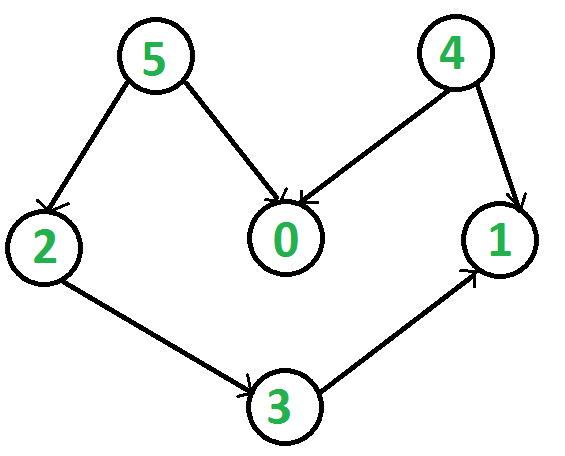
\includegraphics[width=.9\linewidth]{./pic/topologicalSorting.png}
\caption{Topological Sorting}
\end{figure}
\item Topological Sorting vs Depth First Traversal (DFS):
\label{sec-18-2-3-2}
In DFS, we print a vertex and then recursively call DFS for its adjacent vertices. In topological sorting, we need to print a vertex before its adjacent vertices. For example, in the given graph, the vertex ‘5’ should be printed before vertex ‘0’, but unlike DFS, the vertex ‘4’ should also be printed before vertex ‘0’. So Topological sorting is different from DFS. For example, a DFS of the above graph is “5 2 3 1 0 4″, but it is not a topological sorting.
\item Algorithm to find Topological Sorting:
\label{sec-18-2-3-3}
We recommend to first see implementation of DFS here. We can modify DFS to find Topological Sorting of a graph. In DFS, we start from a vertex, we first print it and then recursively call DFS for its adjacent vertices. In topological sorting, we use a temporary stack. We don’t print the vertex immediately, we first recursively call topological sorting for all its adjacent vertices, then push it to a stack. Finally, print contents of stack. Note that a vertex is pushed to stack only when all of its adjacent vertices (and their adjacent vertices and so on) are already in stack.
\end{enumerate}

\chapter{Data Structure}
\label{sec-19}
\section{Easy}
\label{sec-19-1}
\subsection{Two Sum III}
\label{sec-19-1-1}
Design and implement a TwoSum class. It should support the following operations: add and find.
\begin{itemize}
\item add - Add the number to an internal data structure.
\item find - Find if there exists any pair of numbers which sum is equal to the value.
\end{itemize}
For example,
\lstset{language=java,label= ,caption= ,numbers=none}
\begin{lstlisting}
add(1); add(3); add(5);
find(4) -> true
find(7) -> false
\end{lstlisting}
\textbf{Tags:} Hash Table, Data Structure

\subsection{Min Stack}
\label{sec-19-1-2}
Design a stack that supports push, pop, top, and retrieving the minimum element in constant time.
\begin{itemize}
\item push(x) -- Push element x onto stack.
\item pop() -- Removes the element on top of the stack.
\item top() -- Get the top element.
\item getMin() -- Retrieve the minimum element in the stack.
\textbf{Tags:} Stack Data Structure
\end{itemize}
\lstset{language=java,label= ,caption= ,numbers=none}
\begin{lstlisting}
public static class MinStack {
    Stack<Integer> stack = new Stack<Integer>();
    Stack<Integer> minStack = new Stack<Integer>();
    public void push(int x) {
        stack.push(x);
        if (minStack.isEmpty() || x <= minStack.peek()) {
            minStack.push(x);
        }
    }

    public void pop() { // java boxing & unboxing, container, object specific methods
        if (stack.peek().intValue() == minStack.peek().intValue()) 
            minStack.pop();
        stack.pop();
    }

    public int top() {
        return stack.peek();
    }

    public int getMin() {
        if (!minStack.isEmpty()) return minStack.peek();
        else return -1;
    }
}
\end{lstlisting}
\section{Hard}
\label{sec-19-2}
\subsection{LRU Cache}
\label{sec-19-2-1}
Design and implement a data structure for Least Recently Used (LRU) cache. It should support the following operations: get and set.
\begin{itemize}
\item get(key) - Get the value (will always be positive) of the key if the key exists in the cache, otherwise return -1.
\item set(key, value) - Set or insert the value if the key is not already
present. When the cache reached its capacity, it should invalidate
the least recently used item before inserting a new item.
\end{itemize}
\lstset{language=java,label= ,caption= ,numbers=none}
\begin{lstlisting}
public static class LRUCache {
    public class Node {
        int key;
        int value;
        Node prev;
        Node next;
        public Node(int x, int y){
            key = x;
            value = y;
        }
    }

    private HashMap<Integer, Node> hash;
    private int cap;
    private int number;
    Node head;
    Node tail;
    public LRUCache(int capacity) {
        cap = capacity;
        number = 0;
        head = new Node(-1, -1);
        head.prev = null;
        head.next = null;
        tail = head;
        hash = new HashMap<Integer, Node>(capacity); // so I can restrict a size !!
    }

    public int get(int key) {
        Node res = hash.get(new Integer(key)); // don't understand here
        if (res != null) {
            refresh(res);   // update usage frequence
            return res.value;
        } else return -1;
        /*
          if (hash.containsKey(key)) {
          //Node res = hash.get(new Integer(key)); // don't understand here
          Node res = hash.get(key);
          refresh(res);   // update usage frequence
          return res.value;
          } else {
          return -1;
          }
        */
    }

    // so still, must maintain a doubly-linked list to order usage frequency
    public  void refresh(Node tmp) {
        if (tmp == head.next) return; // it's head already

        Node temp = head.next;  // head node in the hash
        Node prevNode = tmp.prev;
        Node nextNode = tmp.next;
        // set to be most recently used~~ move the tmp node to be head.next, connections
        head.next = tmp;  
        tmp.prev = head;
        tmp.next = temp;
        temp.prev = tmp;
        prevNode.next = nextNode;
        if (nextNode != null) 
            nextNode.prev = prevNode;
        else tail = prevNode;   // remember tail as well 
    }

    public void set(int key, int value) {
        Node res = hash.get(new Integer(key));
        if (res != null) {
            refresh(res);
            res.value = value;
        } else {
            //if (!hash.containsKey(key)) { // another way of detecting existing
            Node prevNode = new Node(key, value); 
            Node temp;
            if (number == cap) { // remove tail;
                temp = tail.prev;
                hash.remove(tail.key);      // remember to remove from hash too !!!
                if (temp != null) {
                    temp.next = null;
                }
                tail.prev = null;
                tail = temp;
                number--;
            }
            // add to tail first
            tail.next = prevNode;
            prevNode.prev = tail;
            tail = prevNode;
            refresh(prevNode);
            hash.put(key, prevNode); 
            number++;  // count node numbers
        }
    }
}
\end{lstlisting}
\chapter{细节实现题}
\label{sec-20}

\chapter{Math}
\label{sec-21}
\section{Easy}
\label{sec-21-1}
\subsection{Add Binary}
\label{sec-21-1-1}
\subsection{Roman to Integers}
\label{sec-21-1-2}
\subsection{String to Integer (atoi)}
\label{sec-21-1-3}
\subsection{Palindrome Number}
\label{sec-21-1-4}
\subsection{Plus One}
\label{sec-21-1-5}

\subsection{Factorial Trailing Zeroes}
\label{sec-21-1-6}
\subsection{Excel Sheet Column Title}
\label{sec-21-1-7}
\subsection{Excel Sheet Column Number}
\label{sec-21-1-8}
\subsection{Reverse Integer}
\label{sec-21-1-9}
\section{Medium}
\label{sec-21-2}
\subsection{Multiply Strings}
\label{sec-21-2-1}
\subsection{Sqrt(x)}
\label{sec-21-2-2}
\subsection{Divide Two Integers}
\label{sec-21-2-3}
\subsection{Pow(x, n)}
\label{sec-21-2-4}
\subsection{Fraction to Recurring Decimal}
\label{sec-21-2-5}
\subsection{Permutation Sequence}
\label{sec-21-2-6}
\subsection{Integer to Roman}
\label{sec-21-2-7}
\subsection{Next Permutation: Math}
\label{sec-21-2-8}
Implement next permutation, which rearranges numbers into the lexicographically next greater permutation of numbers.

If such arrangement is not possible, it must rearrange it as the lowest possible order (ie, sorted in ascending order).

The replacement must be in-place, do not allocate extra memory.

Here are some examples. Inputs are in the left-hand column and its
corresponding outputs are in the right-hand column.
\lstset{language=java,label= ,caption= ,numbers=none}
\begin{lstlisting}
1,2,3 → 1,3,2
3,2,1 → 1,2,3
1,1,5 → 1,5,1
\end{lstlisting}

\section{Hard}
\label{sec-21-3}
\subsection{Valid Number}
\label{sec-21-3-1}
\subsection{Max Points on a Line}
\label{sec-21-3-2}
% Emacs 24.3.1 (Org mode 8.2.7c)
\end{document}